\documentclass[a4paper, 11pt, twoside, openany, onecolumn, final]{memoir}

\usepackage{style}

\title{\tb{Inteligencia artificial: Práctica $8$}}
\author{Álvaro García Tenorio \thanks{\texttt{\url{alvgar14@ucm.es}}}\and Miguel Pascual Domínguez\thanks{\texttt{\url{miguepas@ucm.es}}}}
\date{\today}

\begin{document}
	\maketitle
	\tableofcontents
	\chapter{Agrupamiento}
	\section{Descripción del conjunto}
	Para este experimento hemos seleccionado un conjunto de datos acerca de las características sobre 3 tipos de semillas diferentes. Los datos pertenecen a un estudio académico realizado por diversos individuos pertenecientes a una de las siguientes instituciones; la universidad de ciencias de la computación y matemáticas de Polonia, la academia de ciencias de Polonia y de la universidad de Tecnología de Polonia.
	
	Los datos, los hemos obtenido de la siguiente pagina, \url{http://archive.ics.uci.edu/ml/datasets/seeds}. El archivo descargado no venía en formato .arff, por tanto hemos tenido que añadir parte del codigo de definición de atributos y de la relación, ya que solamente venía con los datos del estudio. Los datos no se han visto alterados por nuestras modificaciones. Expliquemos ahora los atributos/variables de este conjunto de datos:
	
	\begin{enumerate}
\item Area: área de la semilla, número real.
\item Perimeter: perímetro de la semilla, número real.
\item Compact: compacidad de la semilla se calcula con la siguiente fórmula $C=4*pi*Area/perimeter^2$, número real.
\item LengthKernel: longitud del centro de la semilla, número real.
\item Width: anchura del centro de la semilla, número real.
\item AssymmetryCoefficient: coeficiente de asimetría, número real. 
\item LengthKernelGrove: longitud del la curvatura del centro de la semilla, número real.
\item VarietiesOfWheat: variedades de semilla de trigo: 1-Kama, 2-Rosa and 3-Canadian, variable categórica.
\end{enumerate}
	\section{Parametrización del algoritmo de agrupamiento}
	Veamos ahora como preparamos los datos y las variables para aplicar el algoritmo de agrupamiento jerárquico.
	
	Veamos primero si debemos normalizar o estandarizar las variables. Para ello, basta con ver que el algoritmo jerárquico de agrupamiento y observar que manipula distancias, por tanto lo recomendable es normalizar todas las variables numéricas para que así todas ellas trabajen en el mismo rango. En cambio en el caso de estandarizar, no saldría rentable.  
	
	Decidamos ahora el número de clusters que queremos para nuestro agrupamiento, para ello tenemos que observar que dependiendo de que variable tomamos como principal y dado que todas las variables menos una son numéricas y la otra es categórica; se debe coger la categórica como principal al realizar el clustering con la opción de Classes to clusters evaluation, con lo cual el número de clusters óptimo es el mismo que el número de clases tiene la variable categórica, que en este caso es $3$.
	
	Para elegir el tipo de enlace que se usa en el algoritmo, hemos probado el algoritmo jerárquico con los $3$ posibles enlaces, simple, centrado y completo; y el enlace con el que los resultados del algoritmo salían homogéneos y dignos de estudiar, era con el enlace completo lo cual se debe a que los individuos del conjunto de datos pertenecientes a la misma clase, están muy alejados unos de otros.
	
	\section{Resultados, conclusiones y respuestas}
	Mostremos primero el sumario de weka en la Figura \ref{SumarioClustering}, y después los histogramas de weka en los que hemos añadido una variable llamada cluster, que nos permite observar como estan organizados los clusters a lo largo de todas las variables, (idea obtenida de las recomendaciones y tutoriales de la página de weka); en la Figura \ref{ClusteringHistogramas}.

Comentemos ahora algunos detalles del sumario, se puede observar que el reparto de las instancias entre los clusters, es realmente equitativo, pues dos clusters tienen un $32\%$ de las instancias y el otro tiene el $36\%$ de las instancias, que hacen un total del $100\%$. Además solo se produce un error del $8\%$ en lo que consiste en la asignación de las instancias al correspondiente clusters, ya que observandolo en el sumario vemos que cada clusters corresponde con una tipo de semilla de trigo, el cluster $0$ corresponde con la semilla de tipo $1$, el cluster $1$ con la semilla de tipo $2$ y el cluster $2$ con la semilla de tipo $3$.

Veamos ahora variable por variable, que valores toman en cada cluster, lo cual lo podemos obtener con la ayuda de los histogramas, pues cada cluster, $0$,$1$ y $2$, es un color, azul oscuro, rojo y azul claro.

	Comencemos con el área, en este caso tenemos que los clusters se distribuyen de una manera gradual, ya que las instancias pertenecientes al cluster $2$ están situadas en los valores mas inferiores con unas pocas instancias del cluster $0$, después en los valores medios están las instancias del cluster $0$ con algunas pocas del cluster $1$ y los valores mas altos son todos de instancias pertenecientes al cluster $1$.
	
	El perímetro tiene exactamente una distribución equivalente, los del cluster $2$, valores bajos; el cluster $0$, unos pocos valores bajos y la mayoría valores medios; y el cluster $1$, sobretodo valores grandes y unos pocos con valores medios.
	
	La compacidad de la semilla está mas distribuida pues el cluster $2$ tiene los valores menores, pero el resto se reparte un poco de manera equitativa entre el cluster $0$ y el $1$, pero predominando más los del cluster $1$ en los valores altos.
	
	La longitud del centro tiene la siguiente distribución, el cluster $2$ está junto con el cluster $0$ en los valores mas bajo, y el cluster $1$ ocupa los valores mas altos. 
	
	La anchura del centro tiene la misma distribución que el perímetro y el área.
	
	Con el coeficiente de simetría se produce el efecto inverso, como si cogieras el histograma y lo pusieras en un espejo, es decir, los clusters $0$ y $1$ ocupan los valores mas bajos, y el cluster $2$ ocupa los valores mas altos, a excepción de dos valores del cluster 0 que están en los valores más altos lo cual se podría deducir que son las dos instancias de la clase $3$ que están colocadas mal en los clusters y en vez de estar en el cluster $2$ están en el $0$.  
	
	Y por ultimo la curvatura del centro tiene la misma distribución que la distribución de la longitud del centro.

Ahora queda por comentar la variable que evaluabamos, la variedad del trigo, y asi poder observar que cluster es mas homogeneo y cual tiene mas valores.

Con una cantidad de individuos de $76$, tenemos que el cluster $1$ es el cluster más numeroso a pesar de ser por pocos individuos pues no son mas de $10$ individuos con ninguno de los otros dos clusters.

Además podemos observar que el cluster más homogéneo es el cluster $1$ pues sus individuos solo pertenecen a dos clases la $1$ y la $2$, y además posee casi todos los elementos de la clase $2$. Después el cluster mas inhomogeneo es el cluster $1$ pues esta repartido entre las $3$ clases. 


	\begin{figure}
  		\centering
   		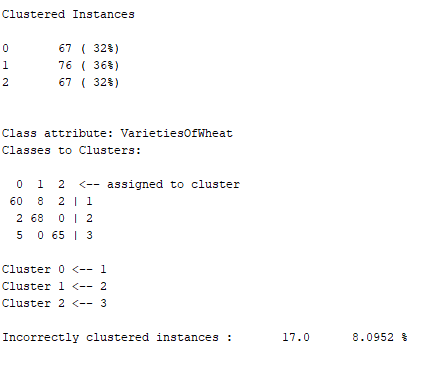
\includegraphics{Imagenes/SumarioClustering}
  		\caption{Sumario Clustering/Agrupamiento}
  		\label{SumarioClustering}
	\end{figure}	
	
	\begin{figure}
  		\centering
   		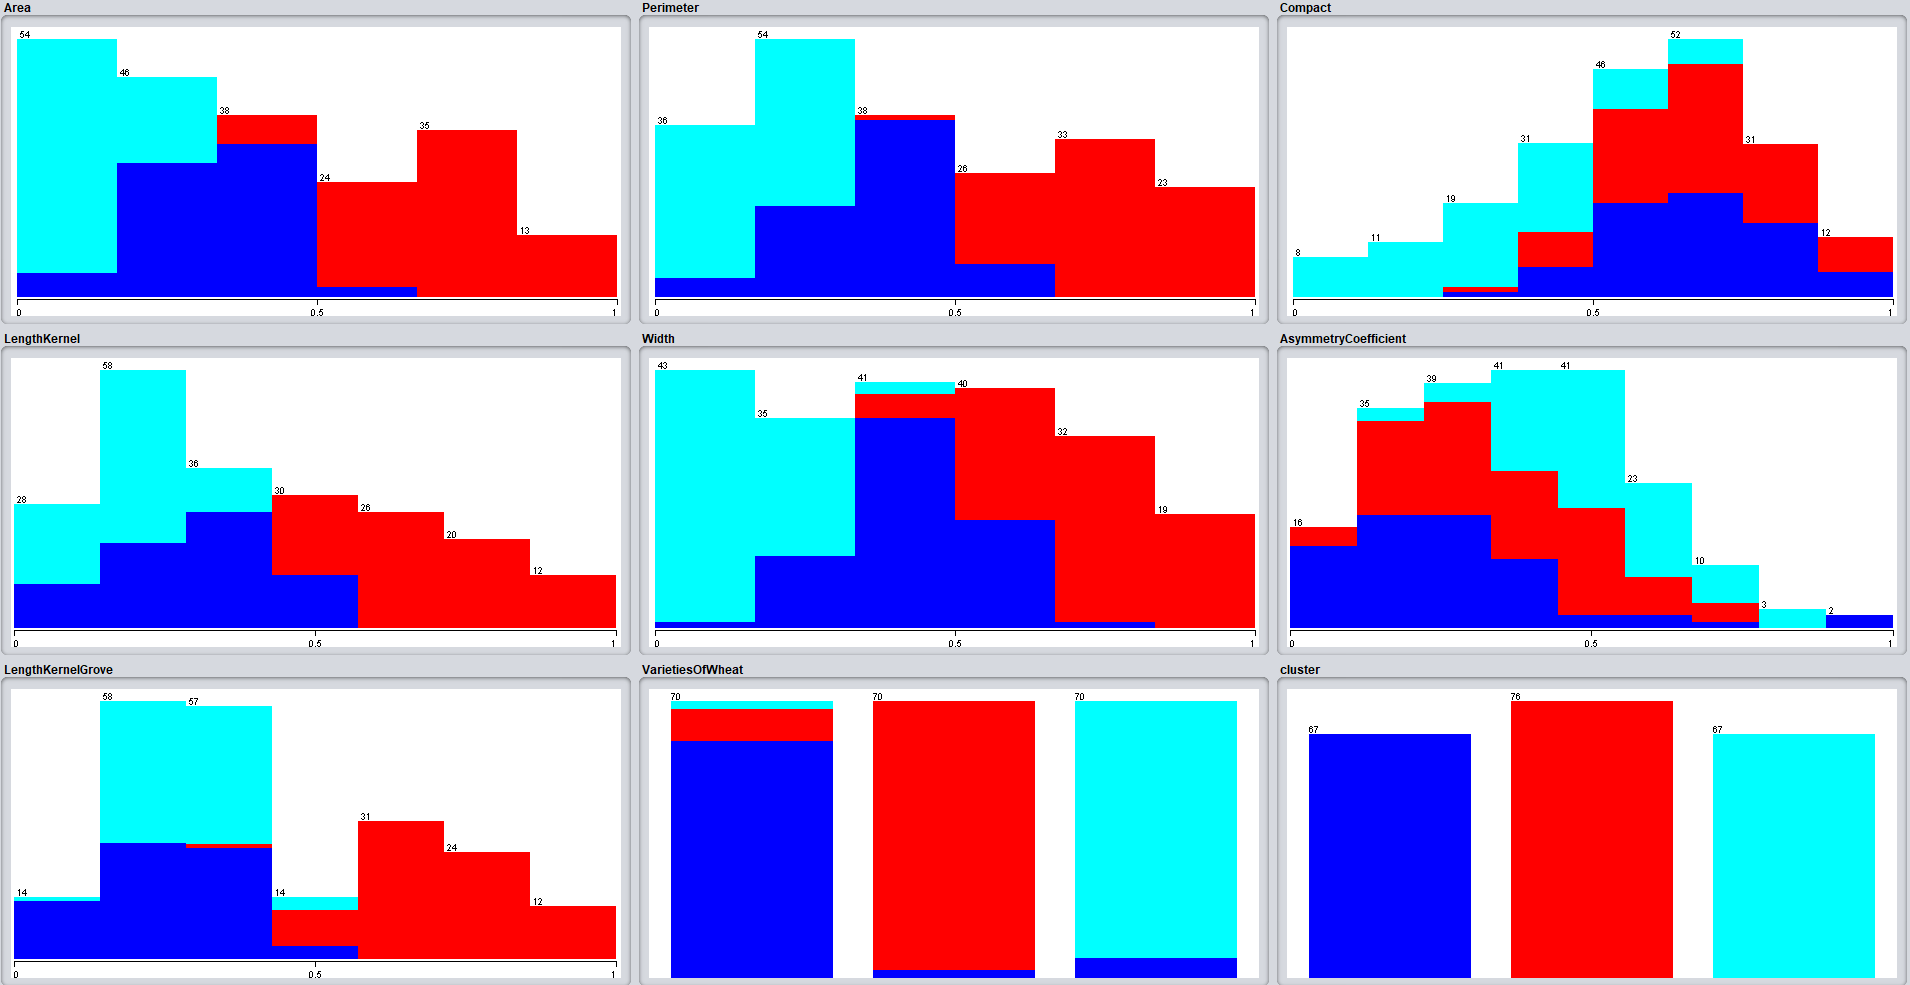
\includegraphics[width=1\textwidth]{Imagenes/Clustering}
  		\caption{Histogramas Clustering}
  		\label{ClusteringHistogramas}
	\end{figure}
	\chapter{Clasificación}
		\section{Descripción del conjunto}
		Para este tipo de problema, lo interesante es coger un conjunto/database que tenga pocos atributos y muchas instancias, por ello el conjunto que hemos seleccionado es un dataset sobre una evaluación de coches, hemos obtenido los datos de la siguiente página \url{http://archive.ics.uci.edu/ml/datasets/Car+Evaluation}. Al igual que en el primer apartado, los archivos descargados no venían en formato .arff, por tanto hemos tenido que añadir parte del codigo de definición de atributos y de la relación, pero los datos no han sido modificados.
		
		Expliquemos ahora los atributos/variables, todos ellos categóricos, ninguno numérico; de este conjunto de datos:
	
	\begin{enumerate}
\item Compra: Precio de compra; muy alto (vhigh), alto (high), medio (med) y bajo (low).
\item Mantenimiento: Precio de mantenimiento; muy alto (vhigh), alto (high), medio (med) y bajo (low).
\item Puertas: Número de puertas clasificado en 4 categorías; 2, 3, 4 y 5 o más.
\item Personas: Número de personas clasificado en 3 categorías; 2, 4 y más.
\item Maletero: Capacidad del maletero; pequeña, media y grande.
\item Seguridad: baja, media y alta. 
\item Tipo de coche según aceptabilidad: inaceptable (unacc), aceptable (acc), bueno (good) y muy bueno (vgood). 
\end{enumerate}
		
		Una vez comentado los atributos, expliquemos el problema. 

Tal y como son los datos, hemos decidido que para aprovechar el potencial de los mismos, lo más lógico es plantear el problema de clasificar la aceptabilidad de los coches en función de los otros 6 atributos, para así poder observar cuales coches son inaceptables y asi no venderlos o comprarlos; ya que así podemos observar más adelante el poder del algunos atributos como la seguridad y el número de personas que ya clasifican una cantidad considerable de los coches.

Mostramos aquí el histograma de la variable tipo de coche según aceptabilidad. 
	\begin{figure}
  		\centering
   		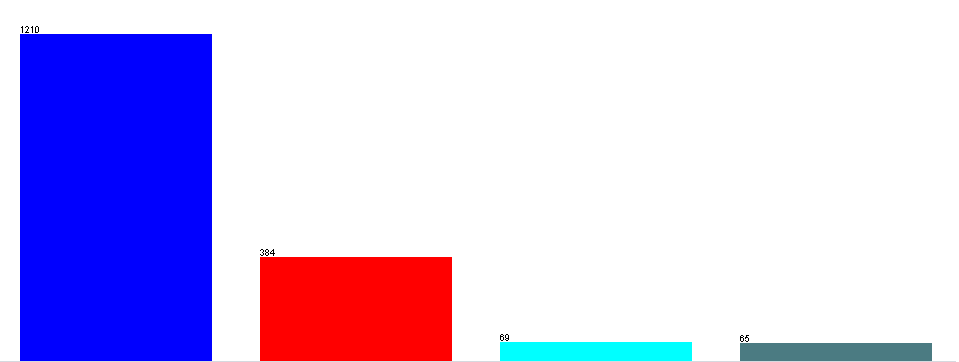
\includegraphics[width=1\textwidth]{Imagenes/HistogramaVarSalidaClasif}
  		\caption{Histograma de la variable tipo de coche según aceptabilidad}
  		\label{HistoVarSalidaClasi}
	\end{figure}
	\section{Parametrización del J48}
		Dado que todas nuestras variables son categóricas no se les puede normalizar (englobar los valores entre $0$ y $1$) ni estandarizar (modificar los datos para que tengan media $0$ y varianza $1$). 
		Primero se realizará una ejecución del algoritmo sin validación ni entrenamiento, después se realizará otra ejecución en validación y entrenamiento al $66\%$.
		
		En la primera ejecución se han mantenido los parámetros del algoritmo predeterminado por Weka y en la segunda ejecución al realizar un entrenamiento y una validación al $66\%$, vimos que el árbol resultante era muy parecido al original sin entrenamiento ni validación, por tanto decidimos añadir una nueva peculiaridad a esta segunda ejecución y era que de manera forzada siempre se realizaran particiones binarias en el árbol, es decir que formara un árbol binario.
	\section{Resultados}
	Mostremos primero los resultados de la primera ejecución, primero mostramos el sumario de weka en la Figura \ref{SumarioPrimeraEjecucion}, en el que esta incluido los valores del recall, precisión los errores y la matriz de confusión; y después el árbol en la Figura \ref{ArbolPrimeraEjecucion}.
	\begin{figure}
  		\centering
   		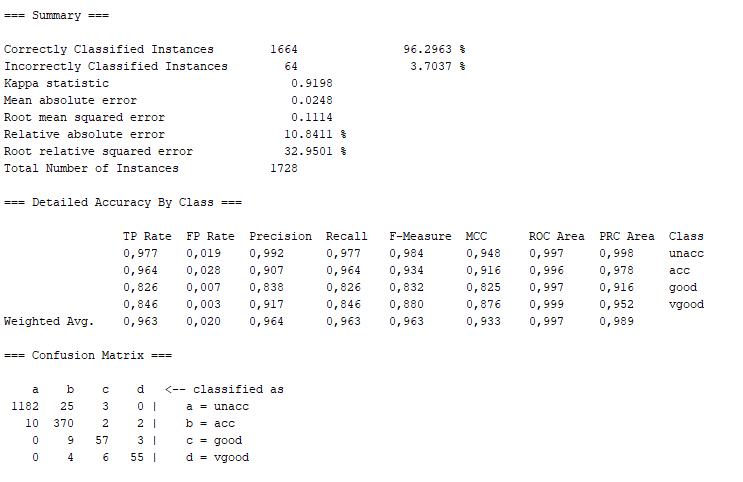
\includegraphics{Imagenes/SummarySinEntreNiVal}
  		\caption{Sumario Primera Ejecución}
  		\label{SumarioPrimeraEjecucion}
	\end{figure}	
	
	\begin{figure}
  		\centering
   		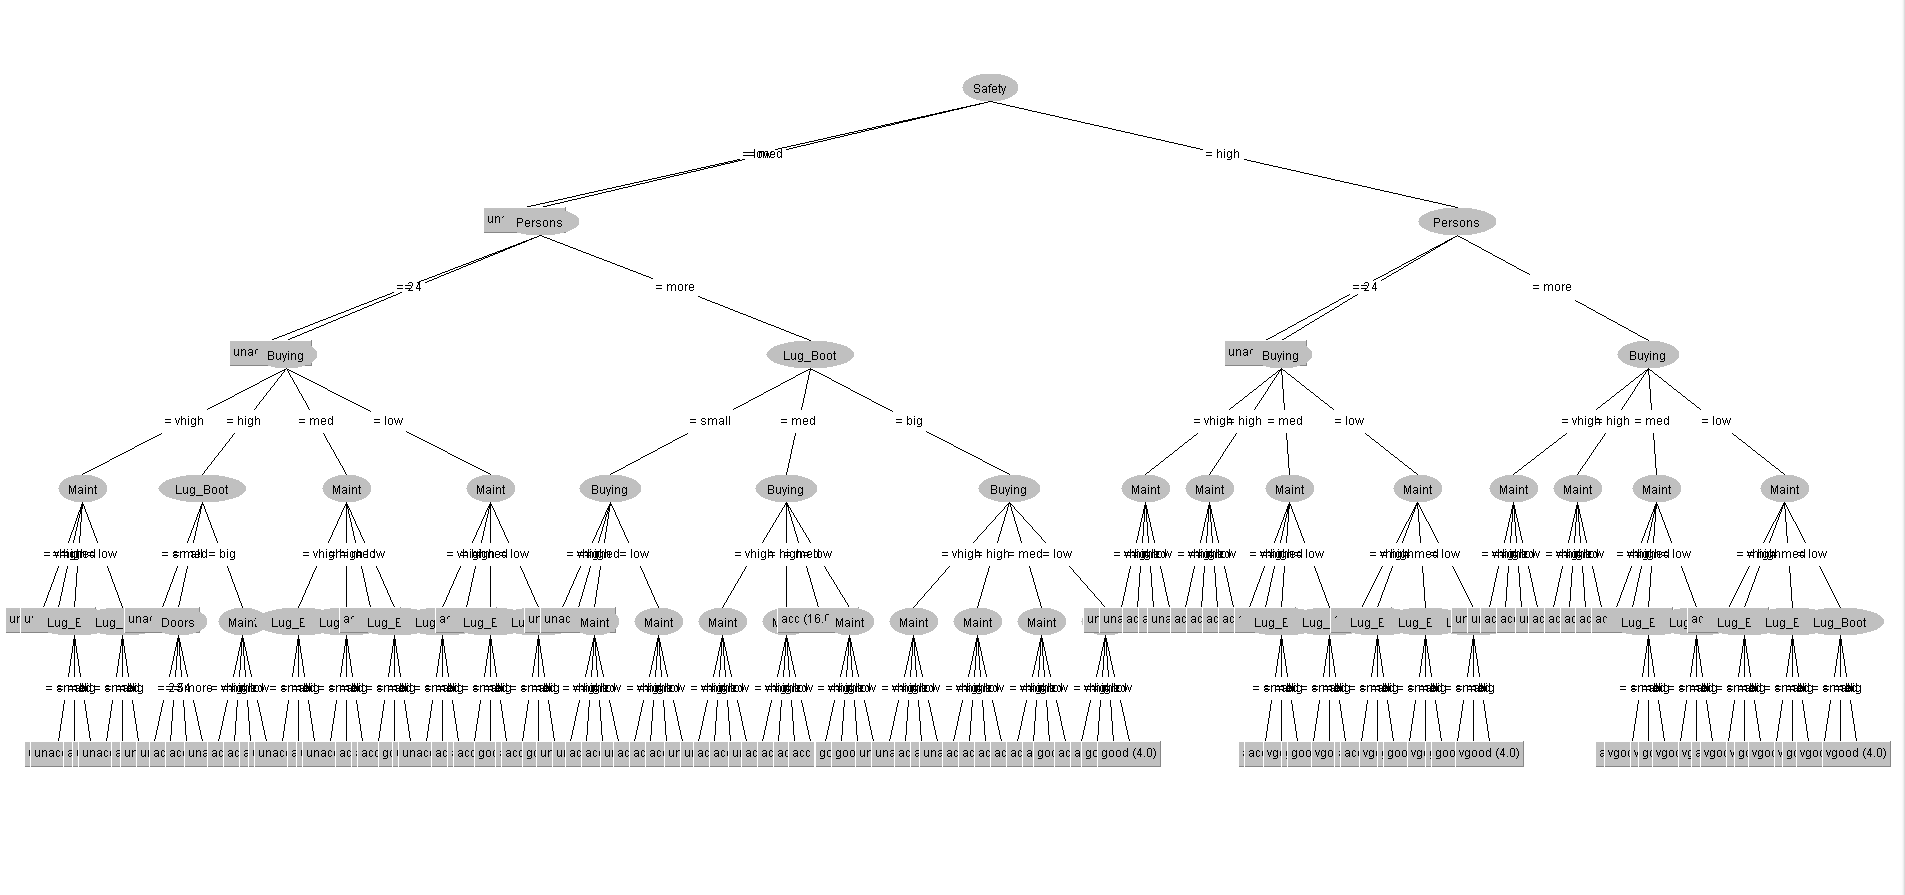
\includegraphics[width=1\textwidth]{Imagenes/ArbolSinEntreNiVal}
  		\caption{Árbol Primera Ejecución}
  		\label{ArbolPrimeraEjecucion}
	\end{figure}
	
	Mostraremos ahora los resultados de la segunda ejecución, primero mostramos el sumario de weka en la Figura \ref{SumarioSegundaEjecucion}, en el que esta incluido los valores del recall, precisión los errores y la matriz de confusión; y después el árbol en la Figura \ref{ArbolSegundaEjecucion}.
	\begin{figure}
  		\centering
   		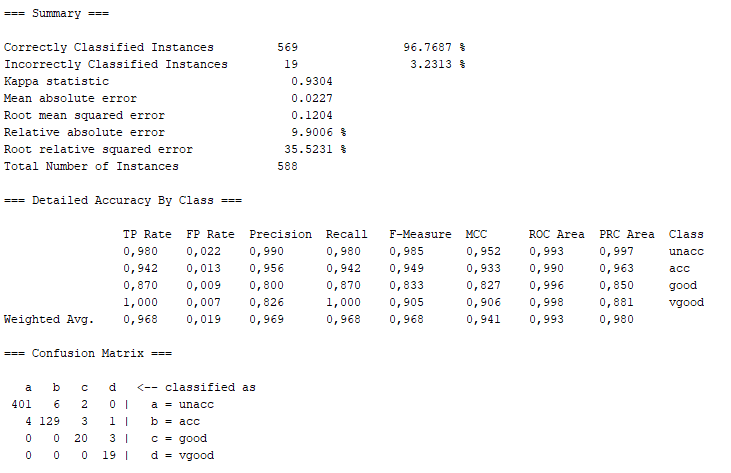
\includegraphics{Imagenes/SummaryConEntreYValYBinarySplit}
  		\caption{Sumario Primera Ejecución}
  		\label{SumarioSegundaEjecucion}
	\end{figure}	
	
	\begin{figure}
  		\centering
   		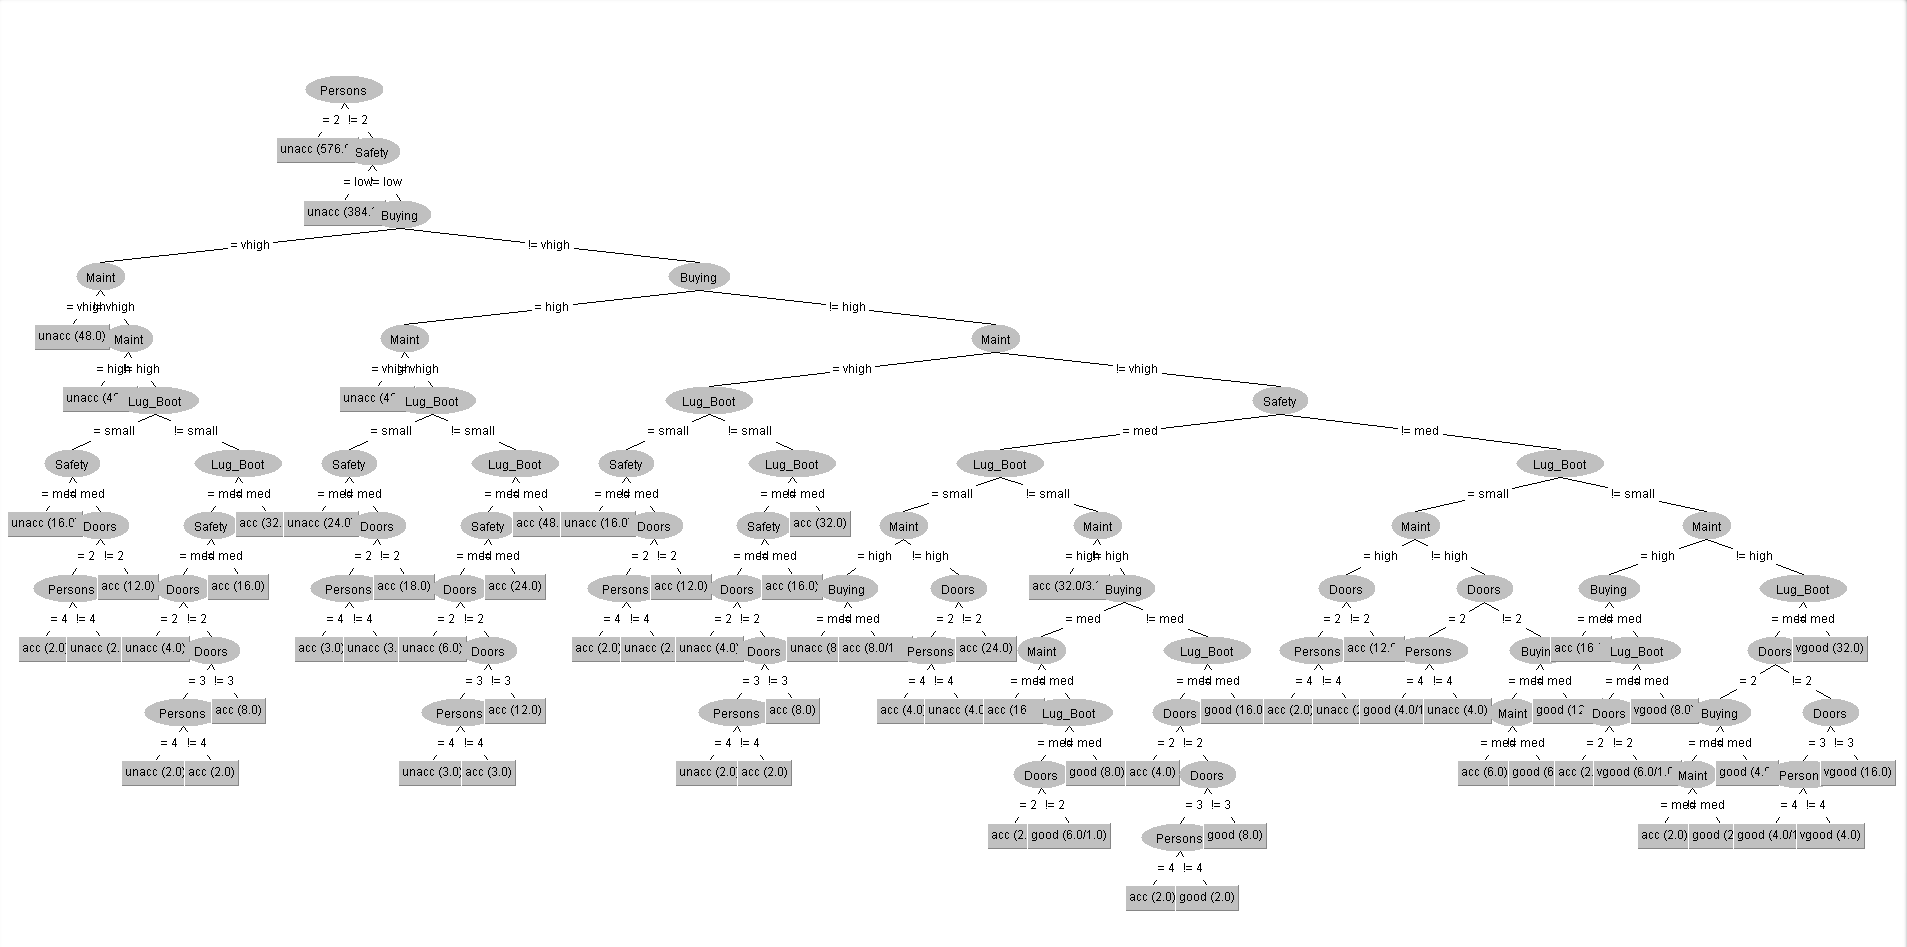
\includegraphics[width=1\textwidth]{Imagenes/ArbolConEntreYValYBinarySplit}
  		\caption{Árbol Primera Ejecución}
  		\label{ArbolSegundaEjecucion}
	\end{figure}
	
	Comentemos ahora los resultados obtenidos en ambas ejecuciones:
	
	Como se puede observar en la primera ejecución se produce un árbol más o menos claro, en el que casi todos los nodos tienen $3$ o $4$ hijos, también se observa que el algoritmo le cuesta diferenciar entre los tipos de coches que son aceptables, buenos o muy buenos; tal y como se ve en la matriz de confusión, también se observa que el porcentaje de instancias mal clasificadas es realmente bajo pues es menor de un $5\%$, lo cual es un porcentaje realmente bueno.
	
	En la segunda ejecución, decidimos forzar a al árbol para que fuera binario, lo que provoca que se cree un  árbol con mayor profundidad y menos homogéneo que el anterior, pero en cambio al realizar una parte de entrenamiento y validación, el porcentaje de fallos en la clasificación es incluso menor, en unas pocas décimas que en la primera ejecución, y además se observa en la matriz de confusión, ahora la confusión que tenía con los coches buenos y muy buenos ha dejado de tenerla. 
	
	En cambio, cabe destacar que a pesar de que la segunda ejecución presenta menos equivocación, la precisión que posee en los coches buenos, es menor que en la primera ejecución, a pesar de que la segunda tiene una precisión global mayor que en la primera ejecución, además de que la segunda parametrización posee una mayor sensibilidad a la hora de concretar en los tipos de coches según aceptabilidad y como es un valor alto y cercano a $1$, sabemos que la validación y ambas ejecuciones son fiables.
	
	\section{Conclusiones y respuestas}
	Por la claridad, y la manera de filtrar que realiza, consideramos que es mejor árbol el de la primera ejecución a pesar de que se confunde en algunas instancias, pero para interpretar el problema, consideramos que se obtiene una interpretación mejor que con la segunda ejecución. Las principales diferencias se encuentran en las ramas iniciales, al ser el primero un árbol con una raíz con mas de dos hijos, hay más claridad y orden en el árbol. 
	
	En cambio en términos de validación consideramos que el segundo árbol es más exacto y con mejores estadísticas que la primera ejecución.
	
	Interpretemos ahora el primer árbol para responder las preguntas en función del contexto del problema.
	
	La raíz del árbol evalúa el atributo de seguridad de un coche, la cual es una de las preguntas mas importantes a la hora de valorar si un coche es aceptable o no, pues un coche seguro es a nuestro punto de vista uno de los vehículos mas peligrosos. Por ello como se puede observar, los coches que mejor ha clasificado y acertado han sido los coches inaceptables (unacc).
	
	Como hemos comentado la seguridad ha sido una de las variables mas relevantes en el problema, además de que es el nodo que más poder discriminante tiene, y a pesar de esto en la segunda ejecución no se ha tomado la seguridad en la raíz sino que se ha tomado el número de personas, a pesar de que están en el mismo nivel, lo cual esto se puede deber al algoritmo de selección interno de weka y que al exigirle la distinción binaria, hace que el número de personas tenga un mayor poder discriminante.   
	
	En efecto, se puede observar que hay dos variables que se confunden sobretodo entre si que son las dos relacionadas con el precio, buying y maint; a lo largo de todo el árbol pues normalmente, son las clases que menos discriminan y se seleccionan las últimas,y que además están organizados con los mismos valores, muy alto (vhigh), alto (high), medio (med) y bajo (low). Tiene cierto sentido que se confundan pues normalmente un coche que cueste mucho dinero, también va a tener un mantenimiento de coste alto. 
	
	Además a nuestro punto de vista, estas dos clases junto con la del tamaño del maletero, son las clases que menos información aportan, pues al final son las que clasifican entre los buenos coches, que si enfocamos este problema simplemente para descartar los coches peligrosos/inaceptables, dichas clases no nos darían información relevante.
	
	\chapter{Regresión}
		\section{Descripción del conjunto}
	\section{Parametrización del perceptrón multicapa}
	\section{Parametrización del K-NN}
	\section{Resultados}
	\section{Conclusiones}
\end{document}